%% Full length research paper template
%% Created by Simon Hengchen and Nilo Pedrazzini for the Journal of Open Humanities Data (https://openhumanitiesdata.metajnl.com)

\documentclass{article}
\usepackage[english]{babel}
\usepackage[utf8]{inputenc}
\usepackage[dvipsnames]{xcolor}
\usepackage{johd}
\graphicspath{ {./images/} }


\title{Annotation Guidelines for Legal Judgment Prediction in Switzerland}

\author{Nina Baumgartner}

\date{} %leave blank
\begin{document}

\maketitle
\section{Introduction}
\subsection{Annotation Goal}
Recently  \citet{Niklaus_2021} presented a diachronic multilingual (German, French, Italian) dataset for \textsc{Legal Judgment Prediction} LJP including 85k Swiss Federal Supreme Court decisions. Using Hierarchical BERT, they achieved a Macro-F1 Score of up to 70\%, considering penal law exclusively, they even achieved a score of up to 80\%. But how accurately can legal experts predict the outcome of a court ruling by just using the facts section of a court case? Do they exceed the performance of the model in accuracy?

This annotation task has the goal to gather these legal expert judgment predictions. In addition, some free text explanations explaining the prediction will also be collected. These guidelines should help you the annotator to use the annotation tool and create consistent annotations. The guidelines you are currently reading are based on the work of \cite{Reiter+2020+193+202}, \cite{Leitner_2019} and \cite{pustejovsky2012natural}. They are a work-in-progress in collaboration with the annotators.

\subsection{Dataset}
The SJP dataset is split into training, validation, and testing set. For this annotation task, an almost balanced subset of the SJP containing 216 cases taken from the test and validation set was created. The dataset is deemed almost balanced because the 216 cases are equally distributed among the three languages contained in the Swiss judicial system German, French and Italian. Each language set contains twelve cases over six years (2015 until 2020). With each year having two cases per legal area\footnote{The chosen legal areas are categorized as penal law, social law and civil law}: One with the verdict approved and one with the verdict dismissed. In addition, we tried to choose one case where the model was correct and one where it was not\footnote{There are some instances of repetitions in the categories, especially in the Italian Dataset. This is why this dataset is only deemed almost balanced}. Cases that were used in the judgment explainability task were discarded from this dataset. The reason is that the annotator may already know the judgment of these cases from the judgment explainability task.

\subsection{Disclaimer}
This document is a work-in-progress. If you have questions or find any errors in these instructions while doing the annotations please feel free to contact the maintainer. Please help with collecting examples to complete these guidelines.

\begin{comment}
% Implementation for the cycles tbd

\section{The Annotation Cycle}
To produce quality annotations and guidelines, which make the annotation task scalable and reproducible the annotations have to be done in cycles. \cite{pustejovsky2012natural} call this process the MAMA (Model-Annotate-Model-Annotate) cycle (see Figure \ref{MAMA_cycle} for details). 

Using the annotation guidelines to identify the correct judgment, multiple annotations by multiple individual annotators are done on the same input. Then these annotations are analyzed and the guidelines are adapted accordingly to provide consistency in the annotations. Therefore, it is important that for the first few cycles the annotations are done individually. Later the gold standard annotations for this corpus will emerge from this process. \cite{pustejovsky2012natural} describe gold standard annotations as the final version of the annotations, which uses the most up-to-date guidelines and has everything labeled correctly. For this work, these gold standard annotations will be done as a team. For the practical aspect of this process please reference section \ref{1_cycle}.

\begin{figure}[H]
    \makebox[\textwidth]{\fbox{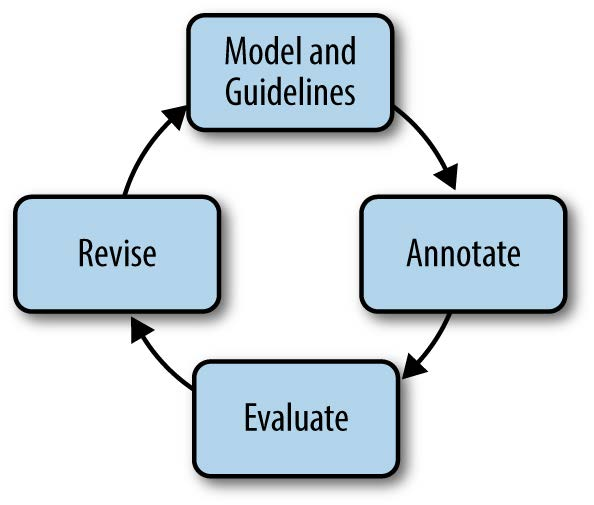
\includegraphics[height=150px]{Annotationguidelines/images/PustejovskyStubbs2013.jpg}}}
     \caption{The inner workings of the MAMA cycle \citep{pustejovsky2012natural}.}
     \label{MAMA_cycle}
\end{figure}
\end{comment}
\section{Annotation Entities}
This section describes the annotation entity you will be annotating by choosing a verdict and giving free text explanation. You will not have access to the entire court document. You should therefore base your decisions only on the text displayed to you by the annotation surface.

\subsection{Fact Section}
The text that you will be annotating is the fact section of a court ruling. The fact section contains the history of the case, legal claims, and the facts themselves. The facts form the foundation for the considerations of the court. This section almost always begins with the word \emph{'facts'} in the respective language of the court case (e.g. \emph{'Sachverhalt'} in German) followed by several subsections which are marked with capital letters. 

After reading the entire text you will annotate it by choosing the appropriate judgment of either \textbf{approved} or \textbf{dismissed} with a single-choice classification. Afterward you will explain why you chose accordingly. There might be cases where you have difficulties annotating. In such a case please reference the coming sections on annotation categories and choose the next most suitable category.

\subsection{Explanations}
\cite{TMTE_2021} identify three types of explanations in the \textsc{Explainable Natural Language Processing} (ExNLP) literature: highlights, free-text, and structured explanations. The explainability annotations for this task consist of structured and free-text explanations. 

There will be a comment section on the annotation interface where you will be writing your explanation in the following structure. Please copy this template to the comment section and add your answers where \$ indicates it.

\subsubsection{Comment Structure}\todo{Add more questions to comment structure?}
\begin{mdframed}[frametitle={\$Annotators name\$}]
Difficulty level for prediction: \$Number between 0-5\$
\begin{itemize}
	\item Why was approval respectively dismissal chosen for this fact section: \$Your explanation\$
	\item Why was this difficulty level chosen: \$Your explanation\$
\end{itemize}	
\end{mdframed}


\section{Annotation Categories}
\cite{Niklaus_2021} explained that originally the cases have been labeled with 6 labels: approval, partial approval, dismissal, partial dismissal, inadmissible, and write-off. To choose a judgment corresponding to a fact section you will have two possibilities. You can either approve a case or dismiss a case. There will be no option to deem a case 'inadmissible' or 'write off', the reason being that cases with this verdict were filtered out of SJP Corpus. Cases with a simultaneous ruling of approval and dismissal in the main request were also excluded from the dataset.\footnote{\cite{Niklaus_2021} describe in their work that in practice, court decisions may have multiple requests (questions), where each can be judged individually. } So you will only read facts from cases where the main request has the same ruling for every sub-request.

In addition, you will be given several options for dealing with problematic cases, which should help to improve the dataset, these guidelines, and the annotations themselves.
\subsection{Approval}
This label is used when a fact section indicates that the request is deemed valid or partially valid respectively (i.e. the court “leans” positive). Please use approval and partial approval as synonyms and annotate a fact section indicating partial approval as approved.
%\todo 1 Add an example

\subsection{Dismissal}
This label is used when a fact section indicates that the request is denied or partially denied respectively (i.e. the court “leans” negative). Please use dismissal and partial dismissal as synonyms and annotate a fact section indicating partial dismissal as dismissed.
%\todo 2 Add an example
\subsection{Problematic Cases}
Problematic cases can occur. For now, we differentiate between two possible types of such cases.

\subsubsection{Rejected Cases}
If a case is badly tokenized\footnote{Tokenized means that the system did not properly separate the words.} or there is another formal error it should be rejected. Please state your reasoning in the comment window using the comment pattern below and reference the \nameref{reject-ignore-case} section of this document for the details on how to properly reject a case. 

\subsubsection{Ignored Cases}
If a case is for some reason unfit for the annotation it should be ignored. To ignore it please state your reasoning in the comment section and follow the steps explained in the \nameref{reject-ignore-case} section of this document below. 

\subsubsection{Comment Structure for problematic cases}\todo{Add more questions to comment structure?}
\begin{mdframed}[frametitle={\$Annotators name\$}]
\begin{itemize}
	\item Why was this case rejected respectively ignored: \$Your explanation\$
\end{itemize}	
\end{mdframed}

\section{Implementation: How to Annotate the Dataset using Prodigy}
This section explains how to use the annotation tool Prodigy\footnote{\href{https://prodi.gy/}{https://prodi.gy/}}. We built a custom recipe for this task which lets you decide on the verdict of a court ruling given only the facts of it.

\subsection{Access}
The Prodigy instance can only be accessed via the University of Bern network. If you want to annotate from home you must use the VPN of the University of Bern\footnote{\href{https://serviceportal.unibe.ch/sp?id=kb_article_view&sysparm_article=KB0010032}{https://serviceportal.unibe.ch/sp?id=kb_article_view&sysparm_article=KB0010032}}.

If you are connected to the university network you can access Prodigy via one of the URLs in the following three sections. Before you can start you will be asked to provide a \emph{username} and a \emph{password}, which will be given to you by the maintainer of the annotation process. After the login procedure, you should now see an overview  of the case (see figure \ref{overview} below) and you can start with your annotation.

\subsubsection{First cycle}\label{1_cycle}
The following links will be used for your pilot annotations (first iteration). If you completed the annotation on this dataset ignored and rejected cases will be replaced with other cases having the same legal area, year, and judgment. This process is ongoing until we reach 72 accepted cases per language. Note that you should insert your name at the end of the URL (instead of 'name').
\begin{itemize}
\item German case annotations:\href{http://fdn-sandbox3.inf.unibe.ch:14000/?session=name}{http://fdn-sandbox3.inf.unibe.ch:14000/?session=name}
    \item French case annotations: \href{http://fdn-sandbox3.inf.unibe.ch:15000/?session=name}{http://fdn-sandbox3.inf.unibe.ch:15000/?session=name}
    \item Italian case annotations: \href{http://fdn-sandbox3.inf.unibe.ch:16000/?session=name}{http://fdn-sandbox3.inf.unibe.ch:16000/?session=name}
\end{itemize}
Note that sessions can be added dynamically by adding the suffix {\color{blue}/?session=name} to the url.
\begin{comment}
% Implementation for the cycles tbd
\subsubsection{Further Cycles and Corrections}\label{2_cycle}
If you have completed all the pending annotations on the above URLs Prodigy will display a message saying no task is available. This is your indicator to continue to this part of the annotations. Reference the Guideline for recent changes and adapt your annotations accordingly. You can repeat this process with a new session as often as you want (see session management example below).

If you need to do multiple corrections on the same case please add a number behind your link as seen below to distinguish between the sessions:

\begin{itemize}
\item Session 1: \href{http://fdn-sandbox3.inf.unibe.ch:11001/?session=angela1}{http://fdn-sandbox3.inf.unibe.ch:11001/?session=angela1}
\item Session 2: \href{http://fdn-sandbox3.inf.unibe.ch:11001/?session=angela2}{http://fdn-sandbox3.inf.unibe.ch:11001/?session=angela2}
\end{itemize}


\subsubsection{Final Gold Standard Annotations}\label{f_cycle}
After some iterations, you and the other annotator will get together and decide on the final annotation using the below link.
\end{comment}


\subsection{Annotate a fact section}
Figure \ref{overview} displays the annotation surface on Prodigy. To choose the judgment for a facts section click on either 'Approval' or 'Dismissal' in the single choice box (see number [1] in figure \ref{overview}). After choosing your judgment please comment on your decision in the comment section indicated with [2]. If you are happy with your annotation you can accept it by clicking on the green check labeled with [3] in Figure \ref{overview} and save it by pressing the save button in the left corner referenced by the number [4].
To see your progress you can look at the information displayed on the left (see the number [5] on Figure \ref{overview}). Please do not forget to save your progress using the save button [3].

If you want to skip a case because you already annotated it. Please use the accept button [1] to get to the next case.

\begin{figure}[h]
    \makebox[\textwidth]{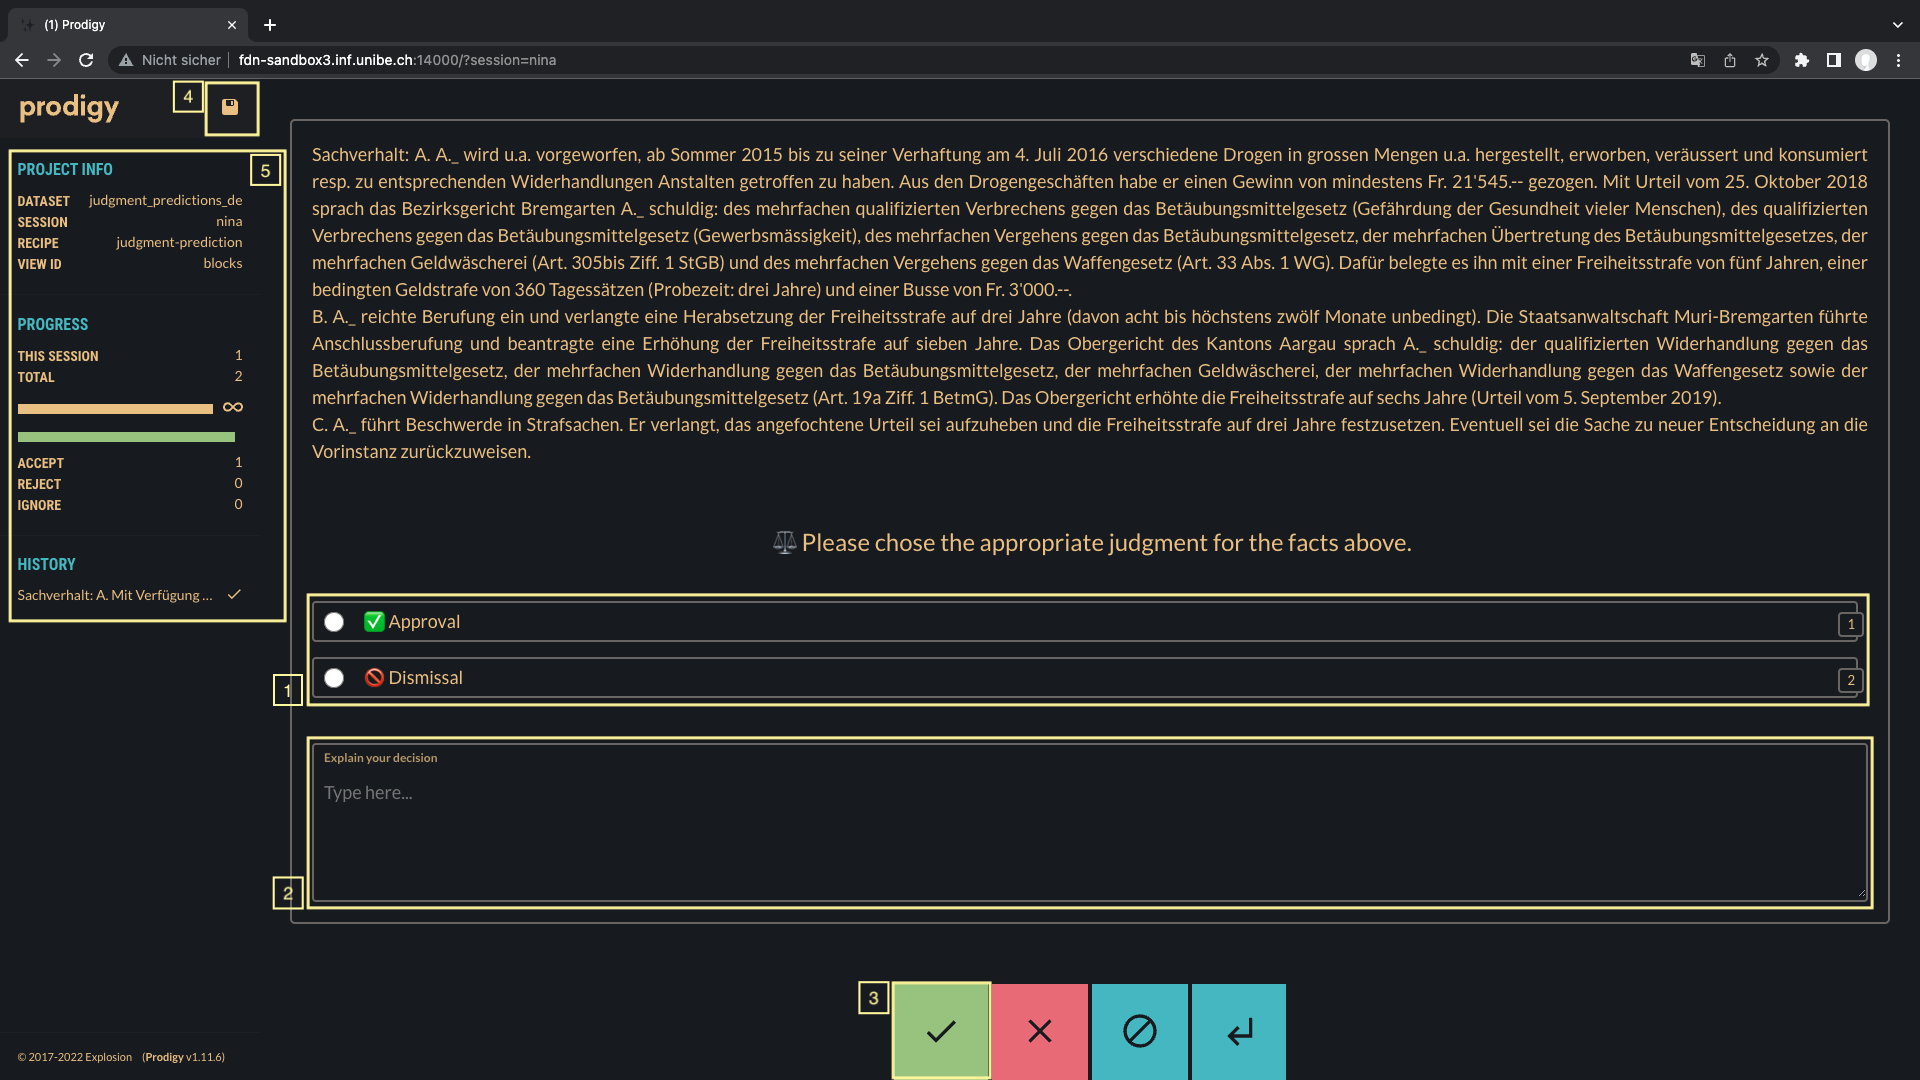
\includegraphics[width=\textwidth]{overview}}
     \caption{Screenshot of the case overview on prodigy}
     \label{overview}
\end{figure}


\subsection{Reject or Ignore a Case}
\label{reject-ignore-case}
To reject a case state your reasoning in the comment section and press the red cross to reject it. To ignore it, press the blue button with the stop signal after commenting. Do not forget to save your progress. Figure \ref{reject_ignore} shows the interface of the comment section and the ignore and reject buttons. 

\begin{figure}[H]
    \makebox[\textwidth]{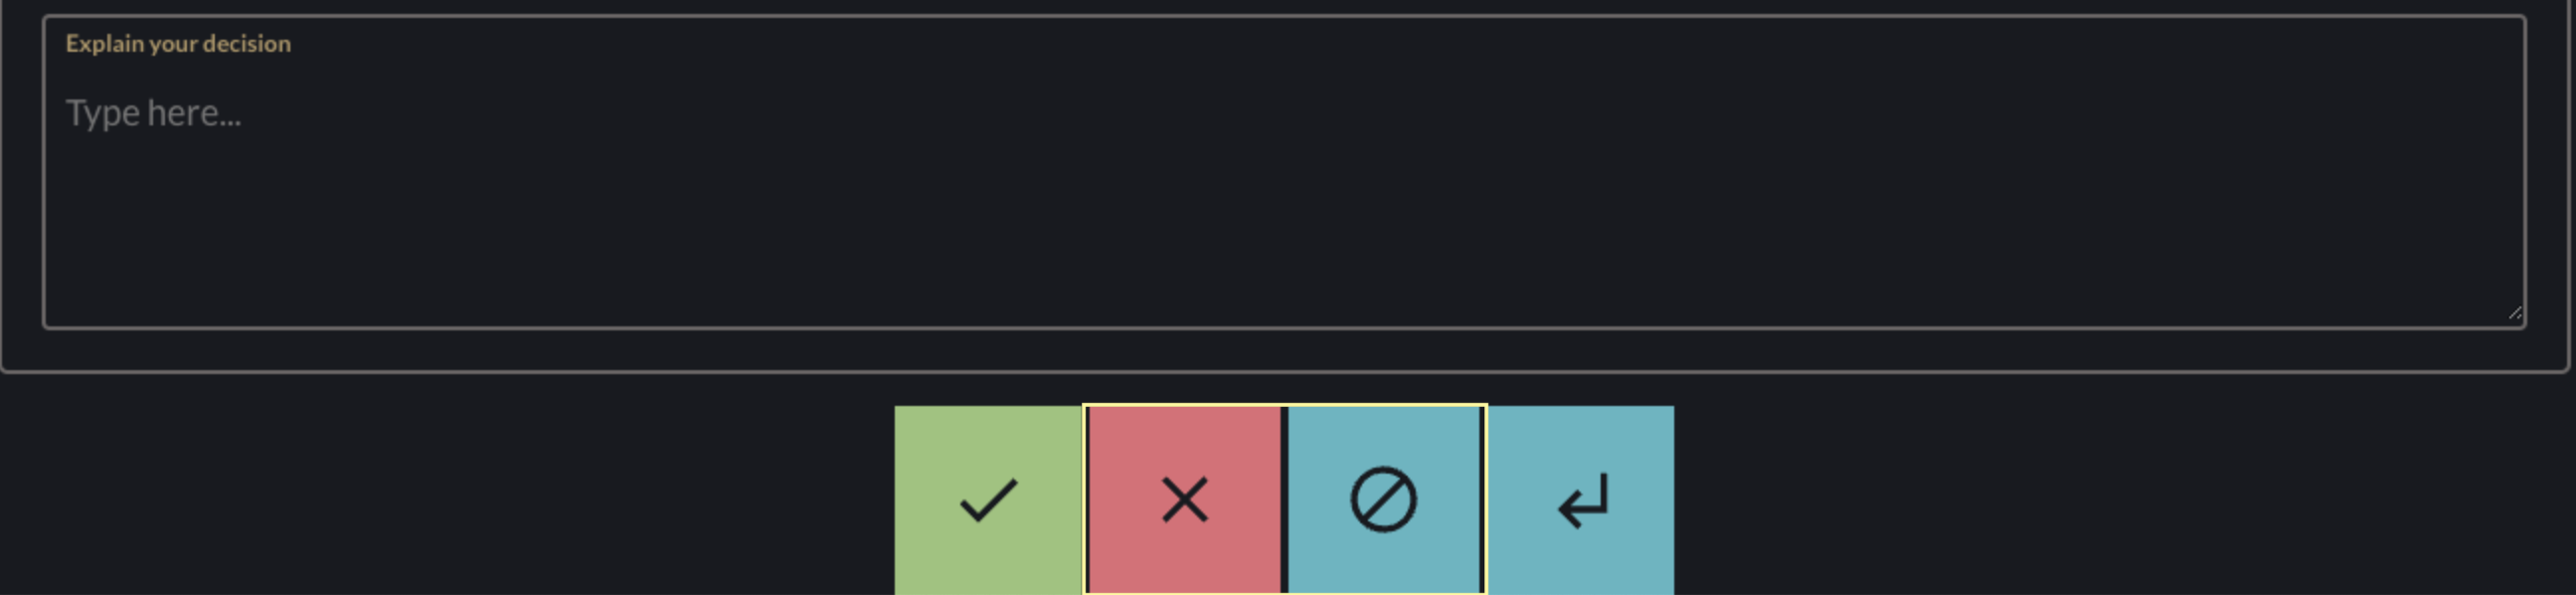
\includegraphics[width=\textwidth]{Annotationguidelines/images/reject_ignore.png}}
     \caption{Reject and Ignore buttons}
     \label{reject_ignore}
\end{figure}

\pagebreak
\section{Change Log}
This change log documents the progress of these guidelines. When adapting these guidelines please also add a new entry to the change log using the following structure
\begin{mdframed}[frametitle={Template}]
\emph{Date – Title of changes}
\begin{itemize}
	\item Which parts were changed in this iteration?
    \item Why was this part changed?
\end{itemize}
\end{mdframed}


\bibliographystyle{johd}
\pagebreak
\bibliography{bib}
\listoffigures


\end{document}